\cleartooddpage[\thispagestyle{empty}]
\chapter{Cerebral Vasculature and the Impact of Disturbed Flow}\label{CHAPTER2}
The human vasculature is a system aimed at carrying blood and lymph through the body. The arteries of the vascular system help deliver oxygenated blood, nutrients, and components such as inflammatory markers and hormones through the body, while the veinous structures help take cellular and tissue waste matter to organs such as the lungs, liver and kidneys for removal as well as carrying deoxygentaed blood back to the heart. The lympahtic vessels transport lymph (fluid containing water and blood cells) to help maintain hemodynamic pressures withing the body. For the purpose of studying IA, the arterial portion of the vasculature will be focused on in this work as the majority of IAs occur within the arterial system. The innermost layer of arteries, known as the tunica intima, is made of a monolayer of endothelial cells (EC) supported by a layer of collagen and elastin. This intimal layer comes into direct contact with the hemodynamic flow environment of the lumen (hollow cavity of the arterial system in which blood flows). Underlying the intima layer is the the tunica media, or media, a layer composed of smooth muscle cells, elastic connective tissue and collagen fibers. The main purpose of the media layer is to contract or dilate the arterial vasculature in response to (as signaled by the intima layer) differing hemodynamic conditions as a means to regulate circulation within the body\cite{bogunovic2019impaired,michel2018genetics}. The outermost layer of arteries, the tunica externa/adventitia, is composed of collagen fibers and elastic tissue helping to maintain the mechanical properties of the vasculature, while the collagen having a secondary purpose of anchoring the vessel to surrounding tissues (improving vessel stability)(Fig.~\ref{Vasculature_Layers}). In terms of vascular changes concerning aneurysm development and rupture, most focus is on changes to the tuinca intima's ECs, and the vascular smooth muscle cells (vSMC) of the tunica media.

\begin{figure}[!h]
  \begin{center}
    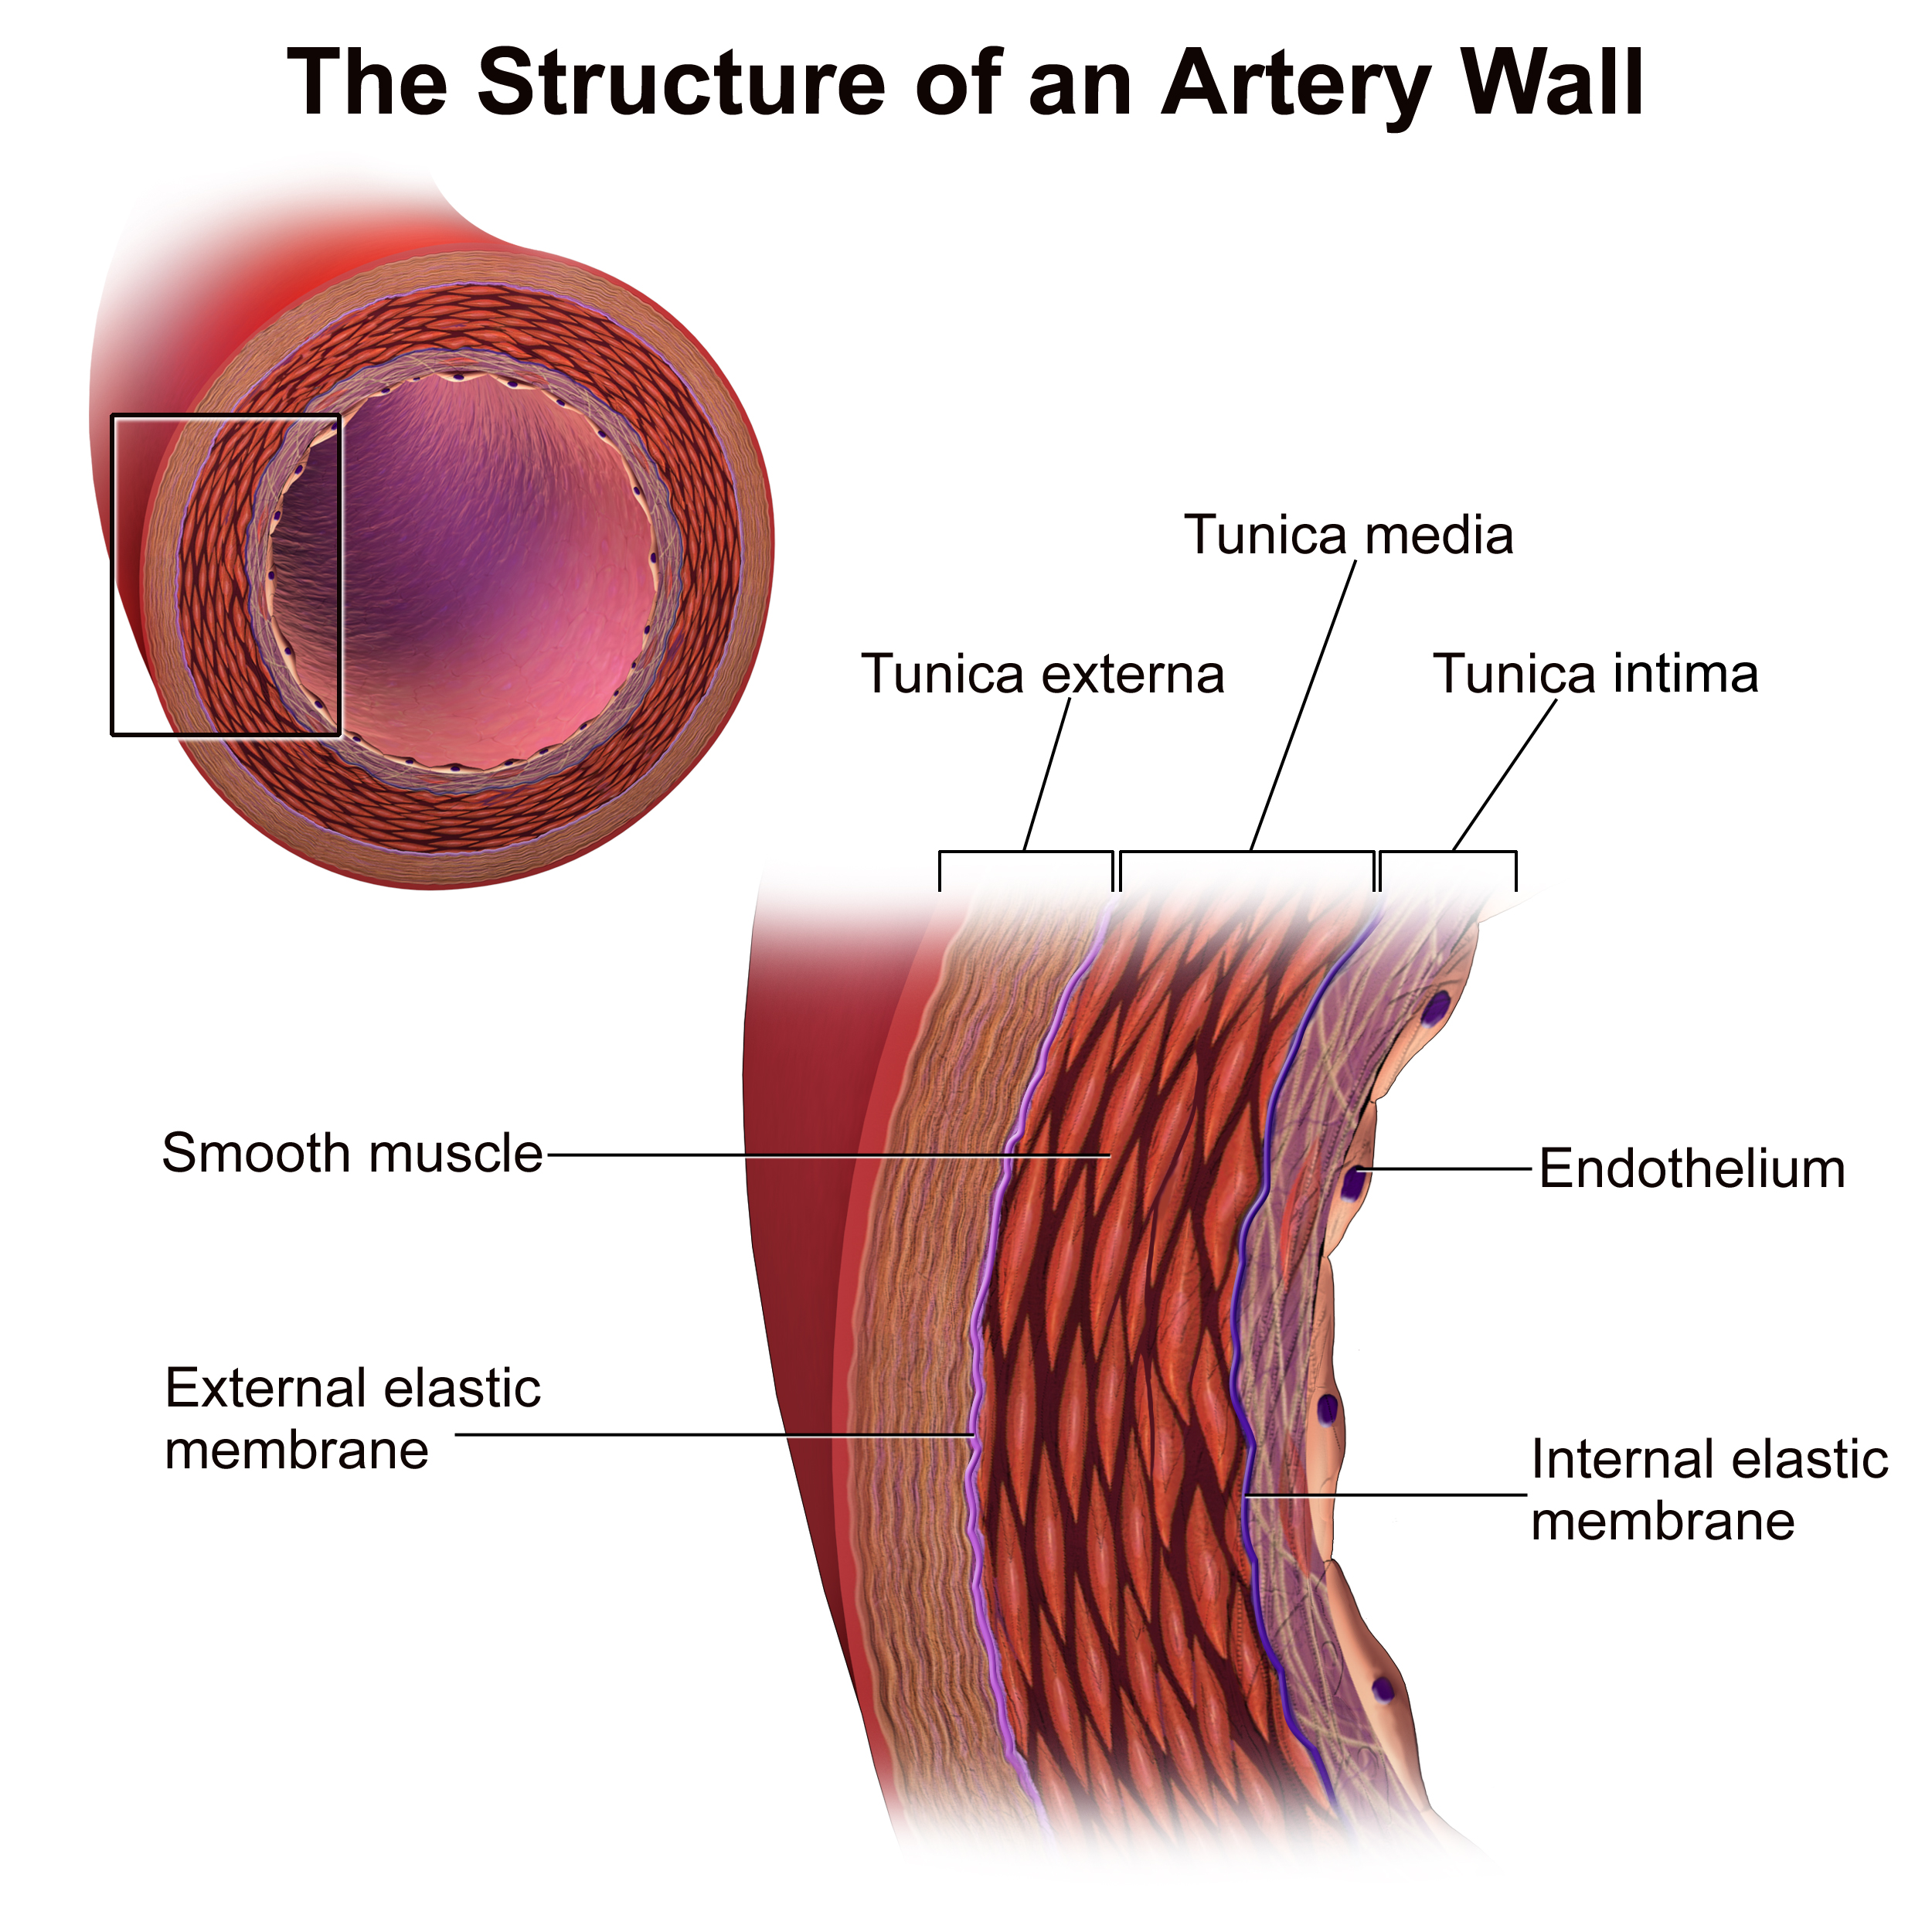
\includegraphics[width=3.5in]{Vasculature}
  \end{center}
  \caption{Layers of the vasculature. Original image from \cite{WIKI_Vessel}}
  \label{Vasculature_Layers}
\end{figure}

\subsection{Endothelial Cells}
ECs are specialized cells that are directly exposed to hemodyanamic environment and its circulating components, with a basolateral surface separated from surrounding tissues by a glycoprotein membrane. Due to ECs direct contact with the hemodynamic environment, their ability to respond to changes in flow conditions is of primary importance. Cytoskeleton actin stress fibers help resist fluid stressors, maintain cellular shape, and aid in cellular mechanotransduction. In laminar flow conditions, actin fibers maintain an oblong orientation, aligning themselves with the direction of flow and forming parallel fibers across the cell to minimize the shear stress exerted by the flowing blood. In addition, ECs act as mechanotransducers, converting mechanincal flow stressors into chemical-cellular signals triggering a variety of cellular processes within the vasculature\cite{CHATZIZISIS20072379}: Cell-cell junctions\cite{dorland2017cell}, caveolae\cite{Shihata2016}, integrins\cite{chien2007mechanotransduction} and the endothelial glycocalyx\cite{cancel2016endothelial}.  Platelet endothelial cell adhesion molecules (PECAM-1) is shown to create bound complexes with integrins\cite{chistiakov2017effects,moriguchi2015pecam}, vascular endothelial growth factor receptor 2(VEGFR-2) and VE-cadherin to transmit shear stressors to cellular responses\cite{chatterjee2018endothelial}. Activated integrins trigger multiple complex of non-receptor tyrosine kinases (FAK, c-Src, Shc, paxillin, and p130CAS), adaptor proteins (Grb2, Crk), and guanine nucleotide exchange factors (Sos, C3G), thereby activating Ras family GTPase.\ref{Mechanotransducers}. EC glycocalyx, membrane-bound proteoglycans, also take part in sensing and transduction mechanical forces into biochemical signals\cite{cooper2017stenosis,mitra2018comparative,cooper2018increased}. Under physiologic laminar flow conditions, glycocalyx triggers an increase in eNOS expression and subsequent NO production\cite{cancel2016endothelial,Frösen2012,zeng2017endothelial}. NO helps regulate vascular dilation/tone and limits vascular inflammation through the inhibition of NF-κB\cite{mcdonald2016glycocalyx,cha2018palmitate} which in turn limits the expression of intercellular adhesion molecule-1 (ICAM-1), a membrane protein involved in vascular adhesion and migration of leukocytes.


\begin{figure}[!h]
  \begin{center}
    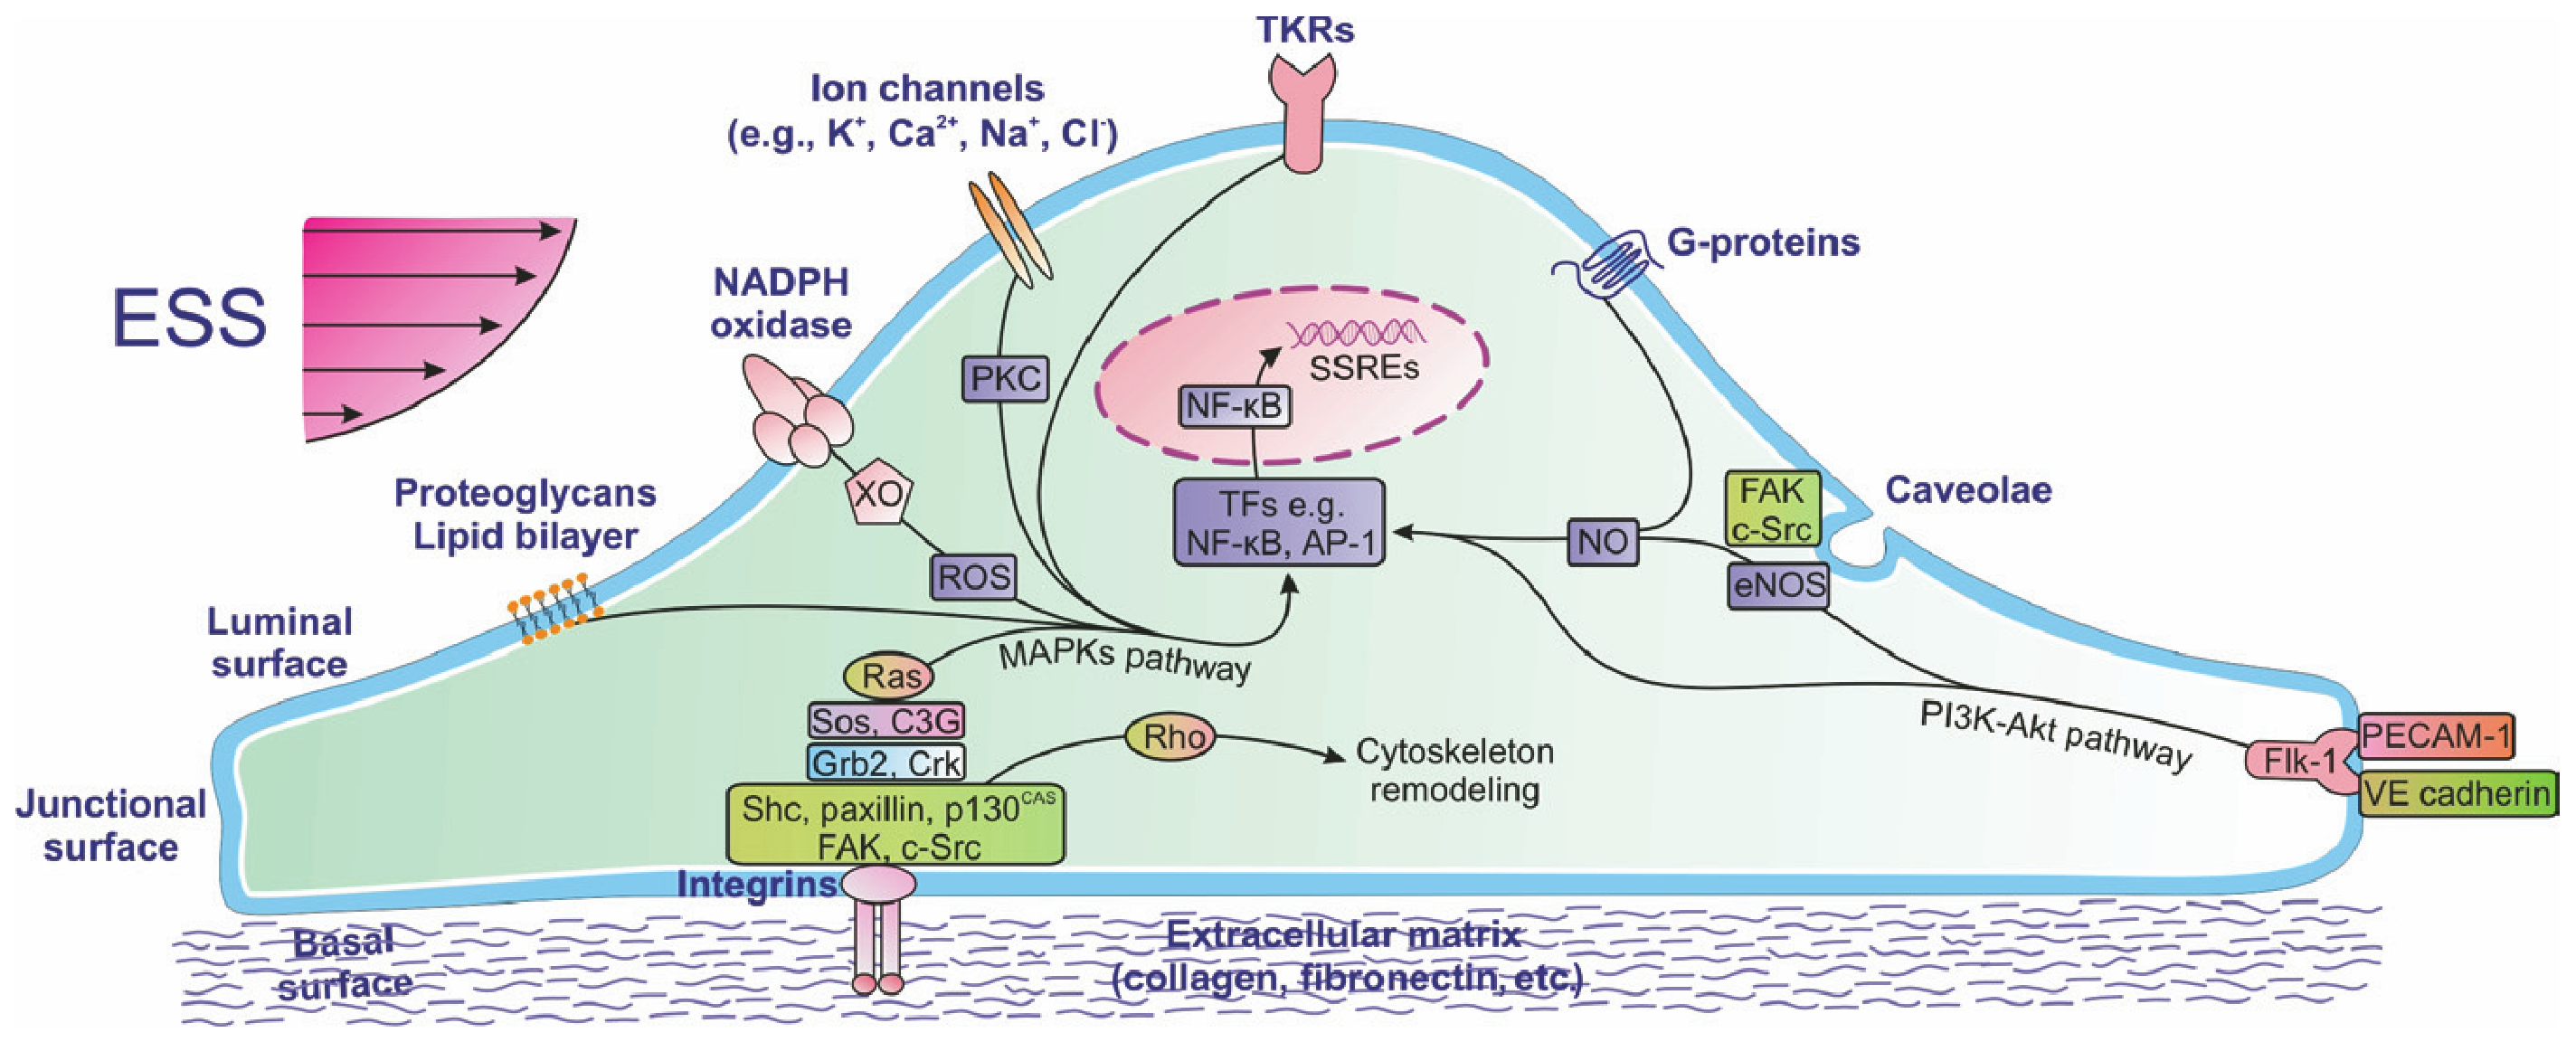
\includegraphics[width=\textwidth]{Mechanotransduction_components.eps}
  \end{center}
  \caption{Mechanoreceptors of ECs: ion channels (K$^+$, Ca$^2+$, Na$^+$, Cl$^-$), G-proteins, caveolae, tryrosiekinase receptors (TKRs), nicotinamide adenine dinucleotide phosphate (NADPH) oxidase, xanthine oxidase (XO), inegrins, and heparan sulfateproteoglycan. Signals are transmitted through the cytoskeleton to the basal or junctional endothelial surface. Integrin mechanosensory complexes consist of platelet endothelial cell adhesion molecule-1 (PECAM-1) and Flk-1. When activated they initiate downstream signaling cascades. Activated integrins trigger multiple complex of non-receptor tyrosine kinases (FAK, c-Src, Shc, paxillin, and p130CAS), adaptor proteins (Grb2, Crk), and guanine nucleotide exchange factors (Sos, C3G), thereby activating Ras family GTPase. Active Ras plays a pivotal role in intracellular transduction of signals as it triggers various parallel downstream cascades of serine kinases; each of these activate downstream signals, ultimately activating mitogen-activated protein kinases (MAPKs). Shear stressors also activate a number of other downstream signaling pathways that impact reactive oxygen species (ROS): NADPH oxidase, activation of protein kinase C (PKC), activation of Rho family small GTPases (mediate the EC remodeling), release of endothelial nitric oxide synthase (eNOS) and activation of phosphoinositide-3 kinase (PI3K)-Akt cascade. These signaling pathways lead to phosphorylation of transcription factors (TFs) such as nuclear factor-kappa(NF-$\alpha\beta$) and activator protein-1(AP-1). Original figure from\cite{CHATZIZISIS20072379}} 
   \label{Mechanotransducers}
\end{figure}


Another role of vascular ECs is the establishment and maintenance of a selective permeability layer within the vasculature\cite{claesson2015vascular,cahill2016vascular}. The outward adventitial interstitial pressure (outside the vasculature) is low, roughly 10mmHg, with a much greater intraluminal arterial blood pressure at ~130/80mmHg (in humans)\cite{stanger2019surgical}. This pressure gradient would create a prominent unidirectional, unchecked mass transport of molecules from the lumen of the vasculature into the surrounding media layer without an additional permeability regulator. The internal EC monolayer helps control macromolecule transport. Typically, maintenance of EC intercellular junctions helps limit macromolecules such as lipoproteins and leukocytes from passing into the intimal layer\cite{gimbrone2016endothelial,Mundi2017}. The main groups of cell-cell complexes that control permeability are adherens junctions\textbf{NEED CITATION} and tight junctions\cite{zhang2016tight}, membrane proteins connected to the cytoskeleton through transmembrane and cytosolic proteins. The proteins of claudins and occludins make up a significant portion of the tight junction between cells\cite{chattopadhyay2014vascular,zhang2016tight}. Tight junctions prevent the passage of molecules and ions through the space between plasma membranes of adjacent cells, so materials must pass enter the cells (by diffusion or active transport) in order to pass through the tissue helping to maintain osmotic balance within the vasculature. Adherens junctions such as vascular endothelial (VE)-cadherin also help cell-cell adhesion (and subsequent EC permeability) well as maintaining an inhibition of endothelial cell growth. A breakdown in these connections leading to \textit{decreased} regulation of permeability within the EC monolayer as 'gaps' now exist between cells, allowing the greater degree of macromolecule infiltration to subsequent layers of the vasculature. While not directly tasked with the maintinance of EC permeability, the regulation of cellular turnover and/or apopotosis has a secondary impact on vascular permeability\cite{qiu2014biomechanical}. Areas of apoptotic cells, or areas of cellular turnover can change the permeability of the vasculature. 

Activated integrins such as $\beta$-1 integrin and integrin $\alpha$5, transmits additional cellular signaling to proteins such as Src homology domain 2-contaning kinase (Shc), which can activate NF-$\kappa\beta$ causing subsequent increases cell proliferation, apoptotic signaling through Jun-amino-terminal kinase (JNK) and altered cellular response to cytokines through p38 mitrogen-activated protein kinase (MAPK). Activated NF-$\kappa\beta$ also triggers downstream activation of a number of genes related to macrophage recruitment and vascular inflammation: MCP‑1, MMP‑2, MMP‑9, IL‑1$\beta$, and inducible nitric oxide synthase(iNOS).


The tunica media of the vasculature is primarily made up of vSMC and produce a significant portion of the vascular extracellular matrix proteins (elastin, collagen, proteoglycans, and fibrillin). This mulit-layered portion of the arterial system help regulate blood vessel integrity and vascular tone in response to hemodynamic forces and are key components in maintaining contractile functionality. Under physiologic conditions, vSMC maintain a nonproliferative phenotype with an abundance of contractile fibers, intermediate filaments, microtubules and actin. Intermediate filaments such as vimentin and desmin aid in the maintenance of vSMC structure[31], whereas microtubules \textbf{DO WHAT}. Actin filaments  transmit mechanical signals dispersed within the vSMC cytoplasm and aid in the transmission of cellular signalling[24]. Changes in cellular tension alter actin cytoskeletal organization, regulating cell contraction, migration and cellular viability[33]. The myosin components within vSMC aid in cellular contraction (similar to actin fibers) and are shown to be altered in the event of vascular injury.

\subsection{Impact of Disturbed Flow on Vascular Cells}
Broadly speaking, the change from a healthy artery to aneurysm development and possible rupture follow an (assumed) overall path: alterations to the ECs, increased macrophage infiltration into the vessel wall, breakdown of proteins (proteolysis) in the extracellular matrix\cite{ramella2018relevance,sawyer2016lymphocytes}, loss of internal elastic lamina\cite{wang2018rabbit,savastano2018biology}, and decreased collagen synthesis\cite{liu2018cyclic,klaus2017association}. Continued pathophysiological conditions can lead to apoptosis of vSMC causing continued weakening of the vascular wall and possible aneurysm formation. In the event of prolonged degradation to the aneurysm wall, an intraluminal thrombosis\cite{di2017hemodynamics,kelsey2017comparison,leach2019relative} or aneurysm rupture may occur.

\begin{figure}[!h]
  \begin{center}
    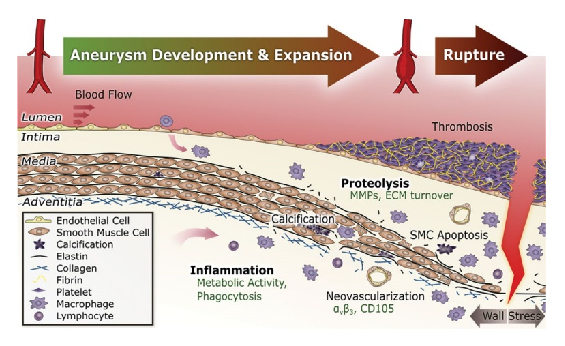
\includegraphics[width=\textwidth]{Artery_healthy_to_rupture.eps}
  \end{center}
  \caption{Schematic representation of abdominal aortic aneurysm (AAA) pathophysiology. Inflammation, proteolysis (breakdown of proteins by enzymes), smooth muscle cell (SMC) apoptosis, neovascularization, calcification, and intraluminal thrombosis may be targeted by molecular imaging. ECM indicates extracellular matrix; and MMP, matrix metalloproteinase.} 
   \label{Artery_to_rupture}
\end{figure}



As mentioned, laminar flow promotes the oblong orientation of actin stress fibers aligned with the direction of flow across the cell in ECs. Low WSS ($<$ 5 dynes/cm$^2$) disturbed flow conditions generated in in vitro, result in altered cytoskeletal orientation with actin fibers forming non-random accumulation at cell peripheries\cite{balaguru2016disturbed,lay2019arhgap18,wong2016parallel}with ECs taking on a round or polygonal shape. Additionally, changes in structural matrix smooth muscle actin expression is reduced in areas of disturbed flow, with lower actin expression in aneurysms versus healthy vessels and further reduction in actin expression within ruptured versus unruptured \cite{aneurysmsvanrossomme2015intracranial}. These alterations to EC morphology 
 





\begin{table}[h]
\caption{Disturbed Flow's Impact on Vascular Cells}
   \centering
   \resizebox{\textwidth}{!}{
\begin{tabular}{|p{70mm}|p{50mm}|l|l|}
\hline
\textbf{Cellular Functionality} & \textbf{Resultant Change due to Disturbed Flow} & \textbf{\textit{Model} Stimulus} & \textbf{Reference} \\
Cellular component/protein & & & \\
\hline
\textbf{Endothelial permeability}& & &\\
VEGF & Increased & & \cite{ashina2015histamine} \\
& Increased & \textit{In-vivo}: CaCl2 induction & \cite{li2017predictive}\\
VEGFR2 & Increased & \textit{In-vitro} Orbital Shaker & \\
VE-cadherin & Decreased & \textit{In-vivo}:ligated arterial segment & \cite{chistiakov2017effects} \\
& Decreased & \textit{In-vitro}: Magnetic twisting & \cite{tsuji2017stagnation} \\
\hline
\textbf{Atherosclerosis} & & & \\
PECAM-1 & Increased & \textit{In-vivo}:ligated arterial segment & \cite{chistiakov2017effects}\\
\hline
\textbf{Mechanotransduction} & & & \\
 $\beta$1-Integrin & Increased & \textit{In-vitro} PPFC& \cite{xanthis2019beta1} \\
Integrin $\alpha$5 & Increased & \textit{In-vitro}: Orbital Shaker & \cite{sun2016activation} \\
Glycocalyx & Decreased & \textit{In-vitro}: PPFC \textit{In-vivo}:Arterial Ligation & \cite{harding2018pro} \\
& Decreased & \textit{In-vivo}:Arterial Ligation & \cite{mitra2018comparative} \\
& Decreased & \textit{In-vitro}: Curved flow chamber & \cite{cooper2018increased} \\
\hline
\textbf{Inflammatory Response} & & & \\
ICAM-1 & Increase & \textit{In-vitro}: PPFC with occulusion & \cite{balaguru2016disturbed} \\
& Increased & \textit{In-vivo}: Arterial LIgation & \cite{sheinberg2019endothelial} \\
& Increased & \textit{In-vitro}: Cone-plate viscometer & \cite{go2014disturbed} \\
& Increased & \textit{In-vitro}: PPFC & \cite{bailey2019mechanoregulation} \\
VCAM-1 & Increased & \textit{In-vivo}: Arterial Ligation & \cite{xanthis2019beta1} \\
& Increased & \textit{In-vitro}: PPFC & \cite{bailey2019mechanoregulation}\\
\hline
\textbf{ECM Remodeling} & & & \\
MMP2 & Increased & \textit{In-vitro}: PPFC with occlusion & \cite{balaguru2016disturbed} \\
& Increased & \textit{In-vitro}: Stenosis flow chamber & \cite{2017stenosis} \\
MMP-9 & Increased &  & \cite{cooper2018increased} \\
\hline
\textbf{Oxidative Stress / Reactive Oxygen Species} & & & \\
NOX & Increased & \textit{In-vivo} genetic knockout/Ang II infusion & \cite{siu2017nox} \\
IL-6 & Increased & \textit{In-vivo}: Arterial Ligation & \cite{sheinberg2019endothelial} \\
& Increased & \textit{In-vitro}: Cone-plate viscometer & \cite{go2014disturbed} \\
IL-1$\beta$ & Increased & \textit{In-vitro}: Cone-plate viscometer & \cite{pan2017shear} \\
IL-5 & Increased & & \cite{baratchi2017molecular} \\
eNOS & Decreased & \textit{In-vitro}: PPFC with occlusion & \cite{harding2018pro} \\
& Decreased & \textit{In-vitro}: Cone-plate viscometer & \cite{bibli2020shear} \\
iNOS & Decreased & \textit{In-vitro}: Orbital Shaker & \cite{mao2014flow} \\
\hline
\textbf{Apoptosis} & & & \\
Caspase 12 & Increase & \textit{In-vitro}: Cone-plate viscometer & \cite{pan2017shear} \\
Caspase 3 & Increase & \textit{In-vitro}: Cone-plate viscometer & \cite{heo2015disturbed} \\
\hline
\textbf{Transcription Factors} & & & \\
NF-$\kappa\beta$ & Increased & \textit{In-vitro}: PPFC & \cite{baeriswyl2019disturbed} \\
& Increased & \textit{In-vitro}: Cone-plate viscometer & \cite{go2014disturbed} \\
Nrf2 & Decreased & \textit{In-vitro}: Orbital Shaker & \cite{martin2014unspliced} \\
JNK & Increased & \textit{In-vivo}: Arterial ligation & \cite{wang2016integrin} \\
& Increased & \textit{In-vitro}: Oscillating stretch of cells on silicone foundation & \cite{codelia2014regulation}\\
 \hline
\end{tabular}}
\label{Distrubed_flow_impact_table}
\end{table}

Docendi eligendi sit et, pri ea dicam eligendi percipitur, has soleat 
dolores convenire te. Sed altera placerat an, id verterem abhorreant 
interesset mea. Eum at ceteros efficiantur. Eos id voluptaria efficiendi 
comprehensam. 

In mel modo dicam vocibus, eruditi consectetuer vim no, cu quaestio 
instructior eum. Justo nostrud fuisset ea mea, eam an libris repudiandae 
vituperatoribus. Est choro corrumpit definitionem at. Vel sint adhuc vocibus 
ea, illud epicuri eos no. Sea simul officiis ea, et qui veri invidunt 
appellantur. Vix et eros ancillae pertinax.

Aliquip lobortis ei est, at error viris graeco sed. Vel te elitr detracto, 
modo graecis scripserit ex nec. Errem utamur viderer per no, eam ea eripuit 
referrentur. Pro te dicat disputando. 

\vspace{0.25in}
\begin{table}[hbt]
  \caption{A portrait table:
    first column represents the year in which the Nobel prize in
    physics was awarded; second column indicates the name of the
    scientist and the third column is the work for which the Nobel
    prize was awareded}
  \begin{center}
    \begin{tabular}{lll}
      \hline
      \multicolumn{1}{c}{\textbf{Year}} & 
      \multicolumn{1}{c}{\textbf{Scientist(s)}} &
      \multicolumn{1}{c}{\textbf{Nobel Work}}\\
      \hline
      1901 & W. C. R\"{o}ntgen & X-rays\\
      1902 & H. A. Lorentz & Influence of magnetism on radiation\\
           & P. Zeeman     & Influence of magnetism on radiation\\
      1903 & A. H. Becquerel & Spontaneous radioactivity\\
           & M. Curie        & Radiation phenomena discovered by Becquerel\\
           & P. Curie        & Radiation phenomena discovered by Becquerel\\
      1904 & J. W. Strutt & Argon\\
      1905 & P. E. A. von Lenard & Cathode rays\\
      1906 & J. J. Thomson & Electrical conductivity of gases\\
      1907 & A. A. Michelson & Spectroscopic and metrological investigations\\
      1908 & G. Lippmann & Photographic reproduction of colours\\
      1909 & K. F. Braun & Wireless telegraphy\\
           & G. Marconi &  Wireless telegraphy\\
      1910 & J. D. van der Waals & Equation of state of gases and liquids\\
      1911 & W. Wien & Laws governing heat radiation\\
      1912 & N. G. Dal\`{e}n & Automatic regulators for lighting coastal beacons\\
           &                 & and light buoys\\
      \hline
    \end{tabular}
    \label{CHAPTER2_TABLE01}
  \end{center}
\end{table}

As explained in Table \ref{CHAPTER2_TABLE01},
Ex offendit elaboraret cum has ex natum honestatis, impedit similique ex duo. 
Et mei mollis scripta, et vim labores phaedrum, in cum facete saperet. 
Splendide elaboraret comprehensam qui ne. Putant verterem no vim, mea solum 
veritus definitiones ei, no labitur propriae deseruisse est. Ius illud everti 
salutandi id, eu facer pericula principes est.

\begin{figure}[htb]
  \begin{center}
    \begin{tikzpicture}[
      thick,
      >=stealth',
      dot/.style = {
        draw,
        fill = white,
        circle,
        inner sep = 0pt,
        minimum size = 4pt
      }
      ]
      \coordinate (O) at (0,0);
      \draw[->] (-0.3,0) -- (8,0) coordinate[label = {below:$x$}] (xmax);
      \draw[->] (0,-0.3) -- (0,5) coordinate[label = {right:$f(x)$}] (ymax);
      \path[name path=x] (0.3,0.5) -- (6.7,4.7);
      \path[name path=y] plot[smooth] coordinates {(-0.3,2) (2,1.5) (4,2.8) (6,5)};
      \scope[name intersections = {of = x and y, name = i}]
        \fill[gray!20] (i-1) -- (i-2 |- i-1) -- (i-2) -- cycle;
        \draw (0.3,0.5) -- (6.7,4.7) node[pos=0.8, below right] {secant};
        \draw[red] plot[smooth] coordinates {(-0.3,2) (2,1.5) (4,2.8) (6,5)};
        \draw (i-1) node[dot, label = {above:$P$}] (i-1) {} -- node[left]
          {$f(x_0)$} (i-1 |- O) node[dot, label = {below:$x_0$}] {};
        \path (i-2) node[dot, label = {above:$Q$}] (i-2) {} -- (i-2 |- i-1)
          node[dot] (i-12) {};
        \draw (i-12) -- (i-12 |- O) node[dot,
          label = {below:$x_0 + \varepsilon$}] {};
        \draw[blue, <->] (i-2) -- node[right] {$f(x_0 + \varepsilon) - f(x_0)$}
          (i-12);
        \draw[blue, <->] (i-1) -- node[below] {$\varepsilon$} (i-12);
        \path (i-1 |- O) -- node[below] {$\varepsilon$} (i-2 |- O);
        \draw[gray] (i-2) -- (i-2 -| xmax);
        \draw[gray, <->] ([xshift = -0.5cm]i-2 -| xmax) -- node[fill = white]
          {$f(x_0 + \varepsilon)$}  ([xshift = -0.5cm]xmax);
      \endscope
    \end{tikzpicture}
  \end{center}
  \caption{Fancy mathematical plots using TikZ package}
  \label{CHAPTER2_FIG02}
\end{figure}

Simul noster voluptaria eam ei, sint regione pri ei. Cum no utinam equidem, 
falli bonorum prodesset an qui. Alterum dissentiet vituperatoribus te eam, 
eos ea suas oblique. Per ea utinam facilisi. Per iudico probatus complectitur 
et, cum tollit atomorum rationibus ea.

Docendi eligendi sit et, pri ea dicam eligendi percipitur, has soleat 
dolores convenire te. Sed altera placerat an, id verterem abhorreant 
interesset mea. Eum at ceteros efficiantur. Eos id voluptaria efficiendi 
comprehensam.

Simul noster voluptaria eam ei, sint regione pri ei. Cum no utinam equidem, 
falli bonorum prodesset an qui. Alterum dissentiet vituperatoribus te eam, 
eos ea suas oblique. Per ea utinam facilisi. Per iudico probatus complectitur 
et, cum tollit atomorum rationibus ea.

\begin{figure}[htb]
  \begin{center}
    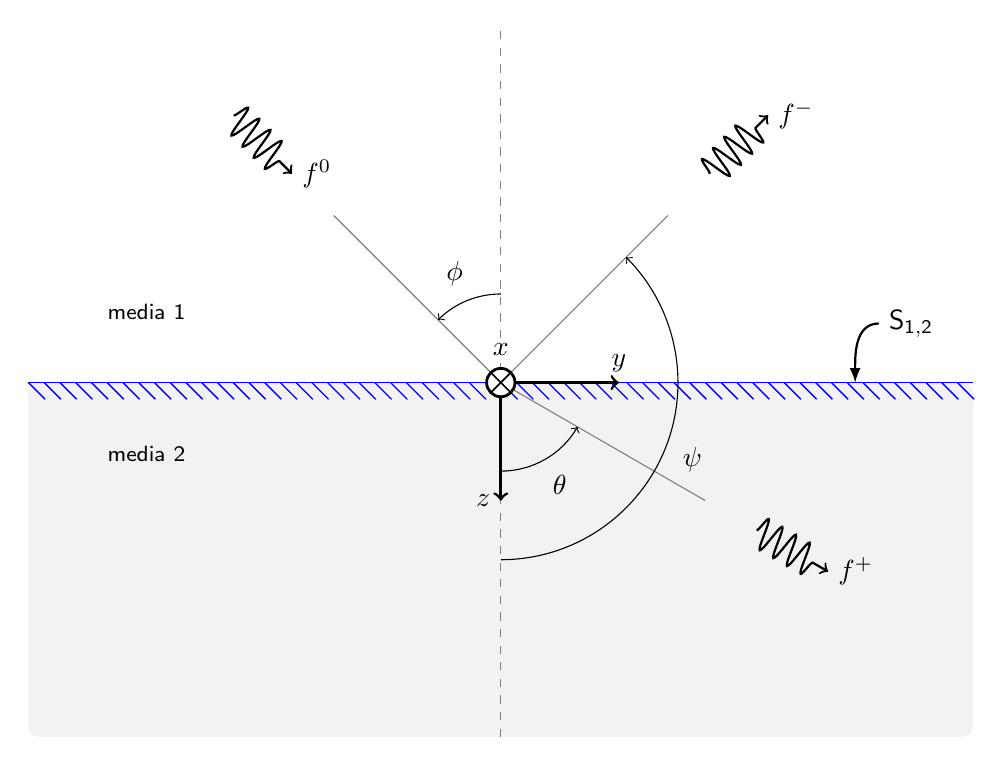
\begin{tikzpicture}[
      scale=1.5,
      media/.style={font={\footnotesize\sffamily}},
      wave/.style={
        decorate,decoration={snake,post length=1.4mm,amplitude=2mm,
        segment length=2mm},thick},
      interface/.style={
        % The border decoration is a path replacing decorator.
        % For the interface style we want to draw the original path.
        % The postaction option is therefore used to ensure that the
        % border decoration is drawn *after* the original path.
        postaction={draw,decorate,decoration={border,angle=-45,
                    amplitude=0.3cm,segment length=2mm}}},
      ]
      % Round rectangle
      \fill[gray!10,rounded corners] (-4,-3) rectangle (4,0);
      % Interface
      \draw[blue,line width=.5pt,interface](-4,0)--(4,0);
      % Vertical dashed line
      \draw[dashed,gray](0,-3)--(0,3);
      % Coordinates system
      \draw(0,0.15)node[above]{$x$};
      \draw[<->,line width=1pt] (1,0) node[above]{$y$}-|(0,-1) node[left]{$z$};
      % Incidence
      \draw[->,wave]
        (135:3.2cm)--(135:2.5cm)node[right]{$f^0$};
      \draw[gray](0:0cm)--(135:2cm);
      \path (0,0)++(113:1cm)node{$\phi$};
      \draw[->](0,0.75)arc(90:135:.75cm);
      % Transmission
      \draw[->,wave]
        (-30:2.5cm)--(-30:3.2cm)node[right]{$f^+$};
      \draw[gray](0:0cm)--(-30:2cm);
      \path (0,0)++(-60:1cm)node{$\theta$};
      \draw[->] (0,-0.75) arc (-90:-30:.75cm);
      % Reflection
      \draw[->,wave]
        (45:2.5cm)--(45:3.2cm)node[right]{$f^-$};
      \path (0,0)++(-22:1.75cm) node{$\psi$};
      \draw[gray](0:0cm)--(45:2cm);
      \draw[->] (0,-1.5)arc(-90:45:1.5cm);
      % Media names
      \path[media] (-3,.6)  node {media 1}
                   (-3,-.6) node {media 2};
      % $x$ axis
      \filldraw[fill=white,line width=1pt](0,0)circle(.12cm);
      \draw[line width=.6pt] (0,0)
        +(-135:.12cm) -- +(45:.12cm)
        +(-45:.12cm) -- +(135:.12cm);
      % Interface pointer
      \draw[-latex,thick](3.2,0.5)node[right]{$\mathsf{S_{1,2}}$}
        to[out=180,in=90] (3,0);
      % To-paths are really useful for drawing curved lines. The above
      % to path is equal to:
      %
      % \draw[-latex,thick](3.2,0.5)node[right]{$\mathsf{S_{1,2}}$}
      %      ..controls +(180:.2cm) and +(up:0.25cm) .. (3,0);
      % Internally the to path is translated to a similar bezier curve,
      % but the to path syntax hides the complexity from the user. 
    \end{tikzpicture}
  \end{center}
  \caption{Incidence, transmission and reflection}
  \label{CHAPTER2_FIG03}
\end{figure}

Docendi eligendi sit et, pri ea dicam eligendi percipitur, has soleat 
dolores convenire te. Sed altera placerat an, id verterem abhorreant 
interesset mea. Eum at ceteros efficiantur. Eos id voluptaria efficiendi 
comprehensam. Simul noster voluptaria eam ei, sint regione pri ei. Cum no 
utinam equidem, falli bonorum prodesset an qui. 
